%
% File lfd1617.tex
%
%% Based on the style files for EACL-2017
%% Based on the style files for ACL-2016
%% Based on the style files for ACL-2015, with some improvements
%%  taken from the NAACL-2016 style
%% Based on the style files for ACL-2014, which were, in turn,
%% Based on the style files for ACL-2013, which were, in turn,
%% Based on the style files for ACL-2012, which were, in turn,
%% based on the style files for ACL-2011, which were, in turn,
%% based on the style files for ACL-2010, which were, in turn,
%% based on the style files for ACL-IJCNLP-2009, which were, in turn,
%% based on the style files for EACL-2009 and IJCNLP-2008...

%% Based on the style files for EACL 2006 by
%%e.agirre@ehu.es or Sergi.Balari@uab.es
%% and that of ACL 08 by Joakim Nivre and Noah Smith

\documentclass[11pt]{article}
\usepackage{eacl2017}
\usepackage{times}
\usepackage{url}
\usepackage{latexsym}
\usepackage{tikz}
\usepackage{pgfplots}
\pgfplotsset{compat=1.14}

%%%% LEAVE THIS IN
\eaclfinalcopy


\newcommand\BibTeX{B{\sc ib}\TeX}



\title{Learning from Data - Assignment 2 - Decision Tree, K-NN}

\author{Remko Boschker \\
  master student of information science at the Rijks Universiteit Groningen \\
  {\tt s1282603, r.boschker@student.rug.nl} }

\date{}

\begin{document}
\maketitle
\begin{abstract}
This study compares the performance of naive Bayes, decision tree and k-nearest neighbour classification of a corpus of reviews by topic. I first investigate what representation of the data works best and find that filtering out stop words works well while the decision tree classifier prefers a count vector instead of a tf-idf vector and the k-nearest neighbour prefers the document to be stemmed versus lemmatised. I next tune the various parameters of the algorithms to find a best f1-score of 0.9087 for the Naive Bayes, of 0.8206 for the Decision Tree and of 0.6644 for the K-nearest Neighbour classification.
\end{abstract}

\section{Introduction}

This study attempts to find the best way to classify reviews by topic. I will analyse the performance of three classification algorithms and for each I will try to find the optimal parameter settings. The algorithms are naive Bayes, decision tree and k-nearest neighbour. I will also analyse what representation of the documents gives the best performance. The representations I want to try are a vector containing the term frequency - inverse document frequency statistic for each word in the document and a sparse matrix containing per document all the counts for all the words in the corpus. For both the vectorisations I will experiment with lemmatisation or stemming of the input words and with a stop word list.

\section{Data}

The study uses a corpus of six thousand product reviews. Each review consists of a label indicating whether the review is positive or negative and a label indicating to which of the followings six topics it belongs: books, camera, dvd, health, music or software. The review also contains a file reference and the actual text of the review. The topic and sentiment labels are distributed almost equally across the corpus. About half of the reviews about a particular topic are labeled positive. Table~\ref{tab:corpus} shows the counts for the labels in the corpus.

\begin{table}[ht]\footnotesize
\caption{counts of topic and sentiment labels}
\label{tab:corpus}
\begin{tabular}{ l r r r r r r }
topic & cnt & \% & pos & \% & neg & \% \\
\hline
books & 993 & 16.5 & 471 & 47 & 522 & 53 \\
music & 1027 & 17.1 & 531 & 52 & 496 & 48 \\
dvd & 1012 & 16.9 & 490 & 48 & 522 & 52 \\
health & 986 & 16.4 & 470 & 48 & 516 & 52 \\
software & 994 & 16.6 & 502 & 51 & 492 & 49 \\
camera & 988 & 16.5 & 504 & 51 & 484 & 49 \\
\hline
total & 6000 & 100.0 & 2968 & 48 & 3132 & 52 \\
\end{tabular}

\end{table}

\section{Method/Approach}

This study compares the performance of the Scikit-learn implementations of three classification algorithms, Multinomial Naive Bayes, decision tree and k-nearest neighbour. First I compare the performance of the algorithms using default parameters but with different representations of the documents that need to be classified. Then I evaluate the effect of tuning the parameters of the algorithms using the best performing document representation. In this way I limit the number of combinations that need to be evaluated. I do not investigate feature selection methods.

I measure the performance in terms of precision, accuracy, f1-score and the time it takes to train and test the models using four-fold cross-validation. I use the cross-validation to predict all topic labels first and then I calculate the scores. The score I use in the evaluation is the weighted average of the scores for the prediction of each of the six labels. The duration is the time it takes for all four cross validation runs to complete training and predicting. The runs are run in parallel on a computer with 16 GB of RAM and a 2.6 GHz quad core Intel i7 processor.

\section{Optimising Representations}

I compare twelve different representations. They are generated using either the tf-idf or count vectoriser from the Scikit-learn Python library. Both vectorisers can be used with or without lemmatisation or stemming and with or without the default stop word list for English included with the library. I use the \emph{PorterStemmer} and \emph{WordNetLemmatizer} from the Scikit-learn library. The \emph{WordNetLemmatizer} requires that the word is tagged as a noun, verb, adjective or adverb. I use the NLTK POS-tagger and then map the resulting Penn Treebank POS-tags to these four categories.

\begin{table*}[ht]\footnotesize
\centering
\begin{tabular}{ l l l l l l l }
vectoriser & preprocessor & stop words & duration & precision & recall & f1-score \\
\hline
tf-idf & lemmatise & english & 2.5min & 0.9113 & 0.9087 & 0.9085 \\
tf-idf & none & english & 1.6s & 0.9089 & 0.9058 & 0.9056 \\
tf-idf & stem & english & 22.8s & 0.9080 & 0.9050 & 0.9048 \\
count & stem & english & 22.5s & 0.9049 & 0.9023 & 0.9022 \\
count & none & english & 1.6s & 0.9045 & 0.9015 & 0.9012 \\
count & lemmatise & english & 2.7min & 0.9038 & 0.9010 & 0.9008 \\
tf-idf & stem & none & 23.4s & 0.9036 & 0.8988 & 0.8986 \\
count & stem & none & 22.9s & 0.9004 & 0.8972 & 0.8972 \\
tf-idf & lemmatise & none & 2.8min & 0.9019 & 0.8968 & 0.8966 \\
count & lemmatise & none & 2.9min & 0.8997 & 0.8955 & 0.8955 \\
tf-idf & none & none & 2.0s & 0.9006 & 0.8953 & 0.8950 \\
count & none & none & 2.2s & 0.8966 & 0.8918 & 0.8916 \\
\end{tabular}
\caption{scores for different representations and the naive Bayes classifier sorted by f1-score}
\label{tab:repres-bayes}
\end{table*}

Table~\ref{tab:repres-bayes} shows the results of running the classification task using the naive Bayes with the twelve document representations mentioned. The results are sorted by f1-score. The difference between the highest and lowest score is only 0.0169. Using stop words to exclude words from the feature vector consistently improves the score by at least 0.0053 and at most 0.0113. Within the scores using the stop words the tf-idf vectoriser performs better than the count vectoriser. Lemmatising improves the score for the tf-idf vectorisation and stemming for the count vectorisation. The lemmatising increases the duration by at least a factor twenty. I will use the highest scoring representation, with a f1-score of 0.9085 for the experiments with parameter tuning. This representation is the tf-idf vectorisation of the lemmatised documents without stop words.

\begin{table*}[ht]\footnotesize
\centering
\begin{tabular}{ l l l l l l l }
vectoriser & preprocessor & stop words & duration & precision & recall & f1-score \\
\hline
count & lemmatise & english & 2.9min & 0.8115 & 0.8073 & 0.8087 \\
count & none & english & 5.0s & 0.8120 & 0.8065 & 0.8081 \\
count & stem & english & 25.6s & 0.8053 & 0.8008 & 0.8023 \\
tf-idf & none & english & 6.0s & 0.8010 & 0.7957 & 0.7974 \\
tf-idf & lemmatise & english & 2.6min &  0.7982 & 0.7940 & 0.7955 \\
count & stem & none & 26.7s & 0.7934 & 0.7917 & 0.7924 \\
tf-idf & stem & english & 25.8s & 0.7939 & 0.7905 & 0.7917 \\
count & lemmatise & none & 2.6min & 0.7926 & 0.7905 & 0.7912 \\
count & none & none & 6.4s & 0.7911 & 0.7870 & 0.7883 \\
tf-idf & stem & none & 29.2s & 0.7773 & 0.7763 & 0.7767 \\
tf-idf & lemmatise & none & 3.1min & 0.7739 & 0.7730 & 0.7733 \\
tf-idf & none & none & 8.1s & 0.7705 & 0.7680  & 0.7689 \\
\end{tabular}
\caption{scores for different representations and the decision tree classifier sorted by f1-score}
\label{tab:repres-tree}
\end{table*}

The results for the decision tree classifier using default parameters are listed in table~\ref{tab:repres-tree}. The difference between the lowest and highest f1-score, 0.0398, is larger than that difference for the Naive Bayes classifier. The stop words improve the score by at least 0.0150 and at most 0.0185. In contrast to the Bayes classifier the decision tree classifier performs better with the count vectorisation. The effect of stemming is not very clear. The highest scoring run used lemmatisation. I will use the representation with the highest f1-score of 0.8087. It is the count vectorisation of the lemmatised document without stop words.

\begin{table*}[ht]\footnotesize
\centering
\begin{tabular}{ l l l l l l l }
vectoriser & preprocessor & stop words & duration & precision & recall & f1-score \\
\hline
tf-idf & stem & english & 23.8s & 0.8073 & 0.8048 & 0.8042 \\
tf-idf & lemmatise & english & 2.6min & 0.7998 & 0.7958 & 0.7953 \\
tf-idf & stem & none & 24.6s & 0.7903 & 0.7837 & 0.7835 \\
tf-idf & none & english & 3.9s & 0.7835 & 0.7780 & 0.7773  \\
tf-idf & lemmatise & none & 2.6min & 0.7767 & 0.7658 & 0.7660 \\
tf-idf & none & none & 4.3s & 0.7489 & 0.7340 & 0.7339 \\
count & stem & english & 23.6s & 0.5627 & 0.5455 & 0.5416 \\
count & lemmatise & english & 2.6min & 0.5555 & 0.5352 & 0.5301 \\
count & none & english & 3.2s & 0.4923 & 0.4775 & 0.4700 \\
count & stem & none &  24.6s & 0.4798 & 0.4622 & 0.4569 \\
count & lemmatise & none & 2.7min & 0.4630 & 0.4520 & 0.4448 \\
count & none & none & 4.3s & 0.4361 & 0.4232 & 0.4158 \\
\end{tabular}
\caption{scores for different representations and the k-nearest neighbour classifier sorted by f1-score}
\label{tab:repres-neighbour}
\end{table*}

Table~\ref{tab:repres-neighbour} lists the results for the k-nearest neighbour classifier. It shows the largest difference in the f1-score for the different representations of the three algorithms. The highest score, 0.8042 is nearly twice the lowest score of 0.4158. The tf-idf vectorisation scores higher than the count vectorisation. The effect of the stop words is less clear than was the case for the other algorithms. Still the two highest scores make use of the stop word list filter. Both vectorisations perform better with the Porter stemmer than with lemmatisation. The best performing vectorisation uses the tf-idf statistic on the stemmed document without stop words and it will be used for the parameter tuning experiments.

All three algorithms perform better when the vector representation of the review documents do not contain any of the stop words in the list included with the Scikit-learn library. Clearly these words are less relevant for classification. The optimal representation for Naive Bayes, lemmatised and using the tf-idf statistic, is what I would expect given that these measure seem to be a more accurate representation of the significant features of a document, because this representation takes into account words that are simply more frequent irrespective of topic and handles morphological differences that I would not expect to be relevant for the semantics. However K-nearest neighbour works better with the documents stemmed and the decision tree works better with the count vectoriser. I cannot explain this result, but would like to note again that the differences is the scores are very small indeed and so perhaps they are not significant enough to draw any conclusions from them.

Comparing the duration of the training and testing without any preprocessing and with default settings (see table~\ref{tab:repres-duration}) shows that Multinomial Naive Bayes is 3 to 4 times faster than a decision tree and twice as fast as k-nearest neighbour while showing the highest scores. However stemming adds about 20 seconds and lemmatising about two and a half minutes. So when using preprocessing the differences between the durations for the algorithms does not seem a relevant factor in preferring one over the other.

\begin{table}[ht]\footnotesize
\centering
\begin{tabular}{ l l l l l l l }
algorithm & vectoriser & duration & f1-score \\
\hline
MB & count &  2.2s & 0.8916 \\
MB & tf-idf & 2.0s & 0.8950 \\
DT & count &  6.4s & 0.7883 \\
DT & tf-idf & 8.1s & 0.7689 \\
KNN & count & 4.3s & 0.4158 \\
KNN & tf-idf & 4.3s & 0.7339 \\
\end{tabular}
\caption{duration of an experiment run without preprocessing}
\label{tab:repres-duration}
\end{table}

\section{Tuning Classification Algorithm Parameters}

In this section I use the optimal representations found in the previous one to investigate the effect of the various tuning options for the three algorithms. I go through all the options that are available for the particular data representation.

\begin{table}[ht]\footnotesize
\centering
\begin{tabular}{ l l l l l l l }
$\alpha$  & fit prior & duration & precision & recall & f1-score \\
\hline
0.9 & false & 3.0min & 0.9114 & 0.9088 & 0.9087 \\
1 & false & 3.3min & 0.9114 & 0.9088 & 0.9086 \\
1.1 & false & 3.2min & 0.9115 & 0.9088 & 0.9086 \\
1 & true & 2.5min & 0.9113 & 0.9087 & 0.9085 \\
0.5 & false & 3.5min & 0.9101 & 0.9082 & 0.9081 \\
0.8 & false & 3.0min & 0.9103 & 0.9078 & 0.9077 \\
0.5 & true & 3.2min & 0.9093 & 0.9073 & 0.9072 \\
1.5 & false & 3.2min & 0.9093 & 0.9073 & 0.9072 \\
1.5 & true & 3.3min & 0.9091 & 0.9057 & 0.9053 \\
0.1 & false & 2.7min & 0.9034 & 0.9028 & 0.9027 \\
\end{tabular}
\caption{scores for different parameter settings of the naive Bayes algorithm}
\label{tab:tune-bayes}
\end{table}

The Multinomial Naive Bayes algorithm takes two parameters, one for the value used in smoothing and one to select whether or not to fit using prior probabilities based on the data. Because the data set has a nearly equal distribution over the topic labels, calculating the prior probabilities does not improve the scoring. Not calculating the priors actually consistently slightly improves the accuracy. Using a smoothing value of 1 is called Laplace and a value between 0 and 1 Lidstone smoothing. 1 and 0.5 are the most common values used. Scores are higher using a smoothing close to one with an interesting exception for 0.5. The highest score uses a value of 0.9. Also here the differences are less than one percent. The scores are listed in Table~\ref{tab:tune-bayes}.


\begin{table}[ht]\footnotesize
\centering
\begin{tabular}{ l l l l }
criterion & splitter & \# features & f1-score \\
\hline
gini & best & none &  0.7964 \\
entropy & best & none &  0.7857 \\
gini & random & none &  0.7967 \\
gini & random & sqrt & 0.5475 \\
gini & random & log2 & 0.4049 \\
\end{tabular}
\caption{scores for different parameter settings for tree construction}
\label{tab:tune-tree-split}
\end{table}

The decision tree classification algorithm supports several ways of influencing how the tree is constructed. You can choose if the algorithm decides on the best split based on the information gain or Gini impurity. You can then determine if that measure is used to alway select the best split or to select the best of a number of random splits. Thirdly you can provide different measures to only consider part of the available feature for the splitting. I ran a few experiments evaluating these parameters. Pre-sorting was not available as an option, because we are using a sparse count vectorisation. Gini appears to perform slightly better than information gain. Random split evaluation can improve performance, but does not give a stable result and makes it hard to evaluate the effect of tuning the parameters for pruning the tree. Not including all the features sharply decreases performance. For the rest of the tuning I use the Gini criterion to find the best split considering all the features. The results are listed in table~\ref{tab:tune-tree-split}.

\begin{table*}[ht]\footnotesize
\centering
\begin{tabular}{ l l l l l l l }
max depth & min for split & min for leaf & max leaves & accuracy & recall & f1-score \\
\hline
5   & 2   & 1  & None & 0.8251 & 0.6035 & 0.6264 \\
20  & 2   & 1  & None & 0.8377 & 0.7903 & 0.7987 \\
50  & 2   & 1  & None & 0.8223 & 0.8107 & 0.8136 \\
60  & 2   & 1  & None & 0.8193 & 0.8097 & 0.8124 \\
75  & 2   & 1  & None & 0.8152 & 0.8088 & 0.8108 \\
100 & 2   & 1  & None & 0.8122 & 0.8077 & 0.8093 \\
50  & 0.1 & 1  & None & 0.8296 & 0.8055 & 0.8096 \\
50  & 10  & 1  & None & 0.8223 & 0.8103 & 0.8134 \\
50  & 5   & 1  & None & 0.8232 & 0.8115 & 0.8143 \\
50  & 4   & 1  & None & 0.8220 & 0.8110 & 0.8137 \\
50  & 5   & 10 & None & 0.8010 & 0.7937 & 0.7957 \\
50  & 5   & 5  & None & 0.8129 & 0.8038 & 0.8062 \\
50  & 5   & 2  & None & 0.8122 & 0.8007 & 0.8033 \\
50  & 5   & 1  & 200  & 0.8297 & 0.8157 & 0.8190 \\
50  & 5   & 1  & 150  & 0.8321 & 0.8172 & 0.8206 \\
50  & 5   & 1  & 100  & 0.8334 & 0.8163 & 0.8199 \\
50  & 5   & 1  & 50   & 0.8410 & 0.8112 & 0.8167 \\
\end{tabular}
\caption{scores for different parameter settings for tree construction}
\label{tab:tune-tree-prune}
\end{table*}


Pruning the decision tree is the process of reducing the size of the tree to make the tree less sensitive to slightly different input values (reduce overfitting). We can set how many times the tree may split, the least amount of samples required for a split, the least amount of samples that should be in a leaf of the tree and the maximum number of leaf nodes. In addition to these there are some settings to handle an uneven distribution of samples.

Limiting the depth of the tree improves accuracy but worsens recall as can be seen in table~\ref{tab:tune-tree-prune}. A balance between the two leads to the highest f1 score when limiting the depth to 50. Looking at the minimum number of samples that should be available to make a split you can see that for a large number of samples, ten percent in the table, leeds to a higher accuracy, but lower recall. Tuning the required sample size for ten and below shows an improvement in both measures simultaneously reaching an optimum at 5. The minimum number of samples required in a leaf node shows the best result for the default value of 1 while the related measure of limiting the number of leaves does show a positive effect at a maximum of 150 leaves.

I expected a similar accuracy - recall tradeoff in parameters limiting the width of the tree as I found for the parameter limiting the depth of the tree, but found none. Perhaps these effects would be clearer if there was no limit set on the depth; something I could evaluate at another time. The duration of the experiments does not really vary with tuning the parameters. It is about three minutes. However using a best random split is about half a minute faster.

The k-nearest neighbours algorithm allows for tuning based on the number of neighbours in the vector space that are looked at to determine the classification. The weight parameter specifies if all neighbours are counted equally in determining the label or if closer neighbours are counted more heavily. Then there are several ways to measure the distance between neighbours. I try Euclidean and Manhattan distance, a Minkowski distance with a power of 2 and 1 respectively. Lastly it is possible to specify the way in which the algorithm searches for neighbours. Although I use tf-idf vectors I can only use brute force search to find the nearest neighbours. The faster \emph{KDTree} and \emph{BallTree} algorithms give an error about sparse features.

\begin{figure}
  \caption{plot of accuracy and f1-score for different values of K}
  \label{fig:tuning-knearest-k}
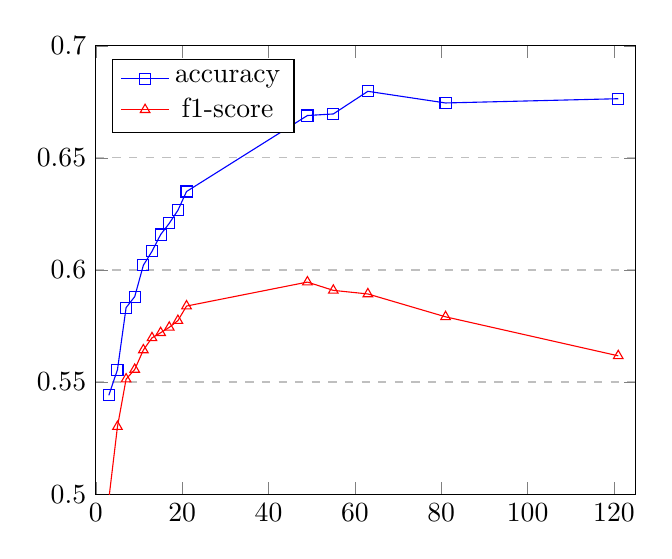
\begin{tikzpicture}

	\begin{axis}[
    title={},
    xlabel={},
    ylabel={},
    xmin=0, xmax=125,
    ymin=0.5, ymax=0.7,
    legend pos=north west,
    ymajorgrids=true,
    grid style=dashed,
	]
  \addplot [
    color=blue,
    mark=square,
    ] coordinates {
    (3,  0.5441)
    (5,  0.5555)
    (7,  0.5832)
    (9,  0.5881)
    (11, 0.6021)
    (13, 0.6083)
    (15, 0.6158)
    (17, 0.6208)
    (19, 0.6266)
    (21, 0.6350)
    (49, 0.6689)
    (55, 0.6696)
    (63, 0.6797)
    (81, 0.6745)
    (121,0.6764 )
  };
  \addlegendentry{accuracy}

	\addplot [
    color=red,
    mark=triangle,
    ] coordinates {
		(3, 0.4978 )
    (5,  0.5301)
    (7,  0.5513)
    (9,  0.5556)
    (11, 0.5643)
    (13, 0.5697)
    (15, 0.5720)
    (17, 0.5744)
    (19, 0.5774)
    (21, 0.5839)
    (49, 0.5946)
    (55, 0.5909)
    (63, 0.5893)
    (81, 0.5791)
    (121, 0.5617)
	};
	\addlegendentry{f1-score}
	\end{axis}
\end{tikzpicture}
\end{figure}

The results for different values of \emph{k} using the default settings for the other parameters are plotted in figure~\ref{fig:tuning-knearest-k}. There is no clear increase of the duration for a larger number of neighbours. The plot shows that for a larger number of \emph{k} the accuracy increases initially but the rate of increase becomes smaller and smaller. There is a remarkable spike of accuracy at \emph{k} equals 63. However the recall starts the go down after \emph{k} becomes larger than 55. The optimum in terms of the f1-score is achieved with \emph{k} at 49. Increasing the number of \emph{k} increases the variance of the system, but decreases its bias and as a result the recall of the system starts to go down; the model has been overfitted.

\begin{table}[ht]\footnotesize
\centering
\begin{tabular}{ l l l l l l l }
weighting & power & duration & f1-score \\
\hline
uniform  & 2 & 2.7min & 0.5946 \\
uniform  & 1 & 3.9min & 0.6380 \\
distance & 2 & 2.8min & 0.6204 \\
distance & 1 & 3.4min & 0.6644 \\
\end{tabular}
\caption{scores for different parameter settings calculating distance to and weight of a neighbour for k=49}
\label{tab:tuning-knearest-dist}
\end{table}

Table~\ref{tab:tuning-knearest-dist} shows the scores for the uniform and distance related weighting (closer is more important) of the labels of the neighbours to determine the class as well as for using the Euclidean and the Manhattan distance. The distance weighting performs better than the uniform one and the Manhattan distance performs remarkably better than Euclidean distance. This is to be expected because the feature vector has a high number of dimensions and a higher Minkowski power puts more emphasis on the largest difference between any two dimensions while a lower power takes more of the dimensions into account. Therefore the Manhattan distance ofter works better than Euclidean distance for high dimensionality vectors.

\section{Discussion/Conclusion}

I explored the tuning options available for the given algorithms and document representation. I am surprised to learn how well the Naive Bayes implementations works for this particular task given that the approach is less complex and makes a strong assumption about the independence of features. It was the fastest, easiest to configure and achieved the highest score. The influence of tuning the different parameters is often very small, but careful preparation of the data representation contributes clearly to a better score. It would be interesting to extend this exploration to include feature selection techniques to evaluate how far you can go in improving the representation of the data set (feature engineering) for a particular classifier.

\section{Answers to additional questions}

\subsection{decision tree theory}

To build the decision tree for the given example with the smallest number of nodes you need to branch on the test with the highest information gain first. Information gain is the expected reduction in entropy for the \emph{edible} label in the example for sorting on either the \emph{color}, \emph{size} or \emph{shape} labels. The information gain is calculated by calculating the entropy for the parent set and subtracting the weighted average entropy of the child sets resulting from splitting on the label. The entropy of a set is calculated by $\sum\limits_i - p_i \log_2 p_i $ where $p_i$ is the probability of an element being in class \emph{i} modeled as the portion of the elements in the set being of class \emph{i}. The information gain achieved by sorting on the \emph{colour, size or shape} features is listed in table~\ref{tab:gain}. Sorting on the \emph{size} first achieves the highest gain and therefore this is what should be done first.

\begin{table}[ht]\footnotesize
\begin{tabular}{ l r r r r r }
& \multicolumn{4}{c}{entropy} & \\
\cline{2-5}
label & parent & child1 & child2 & avg & gain \\
\hline
colour & 0.9886 & 0.9612 & 0.9182 & 0.9531 & 0.0355 \\
size & 0.9886 & 0.8112 & 0.9544 & 0.8828 & 0.1058 \\
shape & 0.9886 & 1 & 0.8112 & 0.9528 & 0.0358 \\
\end{tabular}
\caption{information gain on the first split with respect to the edible label}
\label{tab:gain}
\end{table}



\begin{table}[ht]\footnotesize
\begin{tabular}{ l r r r r r }
& \multicolumn{4}{c}{entropy} & \\
\cline{2-5}
label & parent & child1 & child2 & avg & gain \\
\hline
colour & 0.8112 & 0.6500 & 1 & 0.7375 & 0.0737 \\
shape & 0.8112 & 0.9182 & 0 & 0.6887 & 0.1225 \\
\end{tabular}
\caption{information gain on the \emph{small} branch with respect to the edible label}
\label{tab:gain-small}
\end{table}

\begin{table}[ht]\footnotesize
\begin{tabular}{ l r r r r r }
& \multicolumn{4}{c}{entropy} & \\
\cline{2-5}
label & parent & child1 & child2 & avg & gain \\
\hline
colour & 0.9544 & 0.9852 & 0 & 0.8620 & 0.0923 \\
shape & 0.9544 & 1 & 0.9182 & 0.9387 & 0.0157 \\
\end{tabular}
\caption{information gain on the \emph{large} branch with respect to the edible label}
\label{tab:gain-large}
\end{table}

\begin{figure*}
  \caption{decision tree for predicting edible}
  \label{fig:tree}

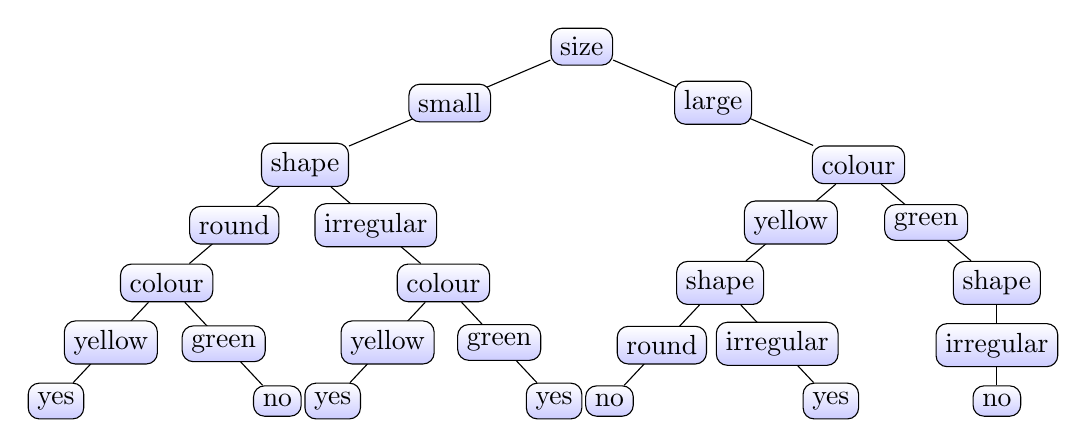
\begin{tikzpicture}[sibling distance=10em,
  every node/.style = {shape=rectangle, rounded corners,
    draw, align=center,
    top color=white, bottom color=blue!20},
  level 1/.style={sibling distance=20em},
  level 2/.style={sibling distance=10em},
  level 3/.style={sibling distance=8em},
  level 4/.style={sibling distance=8em}]
  \node {size}
    child { node {shape}
      child {node {colour}
        child {node {yes}
          edge from parent node {yellow}}
        child {node {no}
          edge from parent node {green}}
        edge from parent node {round}}
      child {node {colour}
        child {node {yes}
          edge from parent node {yellow}}
        child {node {yes}
          edge from parent node {green}}
        edge from parent node {irregular}}
      edge from parent node {small}}
    child { node {colour}
      child { node {shape}
        child { node {no}
          edge from parent node {round}}
        child { node {yes}
          edge from parent node {irregular}}
        edge from parent node {yellow}}
      child { node {shape}
        child { node {no}
          edge from parent node {irregular}}
        edge from parent node {green}}
      edge from parent node {large}};
\end{tikzpicture}
\end{figure*}

As can be seen in the tables~\ref{tab:gain-small} and~\ref{tab:gain-large} for the items labeled \emph{small} the next split with the most gain would be by \emph{shape} and for the items labeled large it would be \emph{colour}. The resulting tree is shown in figure ~\ref{fig:tree}. The leaf for items with the features \emph{yellow,  small, round} has a $\frac{4}{5}$ probability of being edible, but a $\frac{1}{5}$ probability of not being edible. There are no features to distinguish between them. The leaf was labeled with yes, because of the higher probability. The leaf for items with the features \emph{yellow,  large, round} was treated similarly labeling such items as not edible, although there is a $\frac{1}{5}$ probability that the item is edible. There is no item with the features \emph{green, large, round} and no branch for those features is included in the tree.

\bibliography{eacl2017}
\bibliography{yourbibfile}

\end{document}
